\lecture{3}{9. September 2025}{Damping of SDOF systems}

\exercise{3.1}
We consider the shown system, which is to be analyzed as an equivalent SDOF system with the rotation of the rod $\theta(t)$ as the degree of freedom. It is assumed that the rod is uniform, infinitely stiff, has a mass of $m = \qty{3}{kg}$, a length $L = \qty{1,1}{m}$ and does not dissipate mechanical energy. A linear-viscous damping mechanism, which is producing subcritical damping with $\xi = \num{0,2}$ and a spring with stiffness $k = \qty{30}{\frac{N}{m}}$ is applied as shown. The initial conditions are $\theta_0 = 0$ and $\dot{\theta} = \num{0,1}$.

\begin{figure} [ht]
  \centering
  
\includegraphics[width=0.25\linewidth]{./figures/f3_1}
\end{figure}

\paragraph{a)}
Derive the equation of motion for the equivalent SDOF system under the assumption of $LTI$ conditions.
\bigbreak
We imagine the rod being displaced a little to the right at the start since $d_0 > 0$. The force the spring will exert is:
\[ 
F_s = - kL \sin \theta
.\]
And the force that the damper will exert is
\[ 
  F_c = - c \frac{\mathrm{d}}{\mathrm{d}t} \left( \frac{L}{2} \sin \theta \right) = c \frac{L}{2} \dot{\theta} \cos \theta
.\]
The force from gravity will be:
\[ 
F_g = - mg \frac{L}{2} \sin \theta
.\]

Now we take the moments about the support $O$ as:
\begin{align*}
  I_O \ddot{\theta} &= F_s + F_c + F_g \\
                    &= - kL \sin \theta L \cos \theta - c \frac{L}{2} \dot{\theta} \cos \theta \frac{L}{2} \cos \theta - mg \frac{L}{2} \sin \theta \\
                    &= - k L^2 \sin \theta \cos \theta - c \frac{L^2}{4} \dot{\theta} \cos^2 \theta - mg \frac{L}{2} \sin \theta
.\end{align*}
Under $LTI$ assumptions we set $\sin \theta \approx \theta$ and $\cos \theta \approx 1$ and get:
\begin{align*}
  I_O \ddot{\theta} &= - k L^2 \theta - c \frac{L^2}{4} \dot{\theta} - mg \frac{L}{2} \theta \\
 &=  -\theta \left( k L ^2 + mg \frac{L}{2} \right) - c \frac{L^2}{4} \dot{\theta} \\
 \implies I_O \ddot{\theta} + \frac{cL^2}{4} \dot{\theta} + \left( k L^2 + mg \frac{L}{2} \right) \theta &= 0
.\end{align*}
Now inserting the fact that the moment of inertia of a rod rotating about its end is $I_O = \frac{1}{3}mL^2$ we get:
\[ 
  \frac{m L^2}{3} \ddot{\theta} + \frac{cL^2}{4}\dot{\theta} + L \left( kL + \frac{mg}{2} \right) \theta = 0
.\]


\paragraph{b)}
Determine the undamped angular eigenfrequency $\omega_u$.
\bigbreak
For translation we normally have that
\begin{align*}
  m \ddot{d}(t) + c \dot{d}(t) + kd(t) &= 0 \\
  \implies \ddot{d}(t) + \frac{c}{m} \dot{d}(t) + \frac{k}{m} d(t) &= 0 \\
  \implies \ddot{d}(t) + 2 \left( \omega_d \dot{d}(t) + \omega_u^2 d(t) \right) &= 0
.\end{align*}
An analogous result is applicable for rotation, the eigenfrequency is:
\[ 
\omega_u = \sqrt{\frac{k}{m}} \implies \omega_u = \sqrt{\frac{L \left( kL + \frac{mg}{2} \right)}{\frac{m L^2}{3}}}
.\]
This can be simplified as:
\begin{align*}
  \omega_u &= \sqrt{\frac{3L \left( k L + \frac{mg}{2} \right)}{m L^2}} \\
  &= \sqrt{\frac{3 k L + \frac{3mg}{2}}{mL}}
.\end{align*}


\paragraph{c)}
Solve the equation of motion in a) with the given initial conditions and sketch $\theta(t)$
\bigbreak
We have the equation of motion:
\[ 
  \frac{m L^2}{3} \ddot{\theta} + \frac{c L^2}{4} \dot{\theta} + L \left( k L + \frac{mg}{2} \right) \theta = 0
.\]
Now we set $m_{\mathrm{sub}} \equiv \frac{mL^2}{3}$, $c_{\mathrm{sub}} = \frac{c L^2}{4}$ and $k_{\mathrm{sub}} = L \left( k L + \frac{mg}{2} \right)$. Then
\[ 
  m_{\mathrm{sub}} \ddot{\theta} + c_{\mathrm{sub}} \dot{\theta} + k_{\mathrm{sub}} \theta = 0
.\]
The solution of this for undercritial damping is:
\[ 
d(t) = e^{- \xi \omega_u t} \left( A_1 \cos \left( \omega_d t \right) + A_2 \sin \left( \omega_d t \right) \right)
.\]
Where $\omega_d \equiv \omega_u \sqrt{1 - \xi^2}$ and $\xi = \frac{c_{\mathrm{sub}}}{2 m_{\mathrm{sub}} \omega_u}$. We can find an expression for $\xi$ as
\begin{align*}
  \xi &= \frac{c_{\mathrm{sub}}}{2 m_{\mathrm{sub}} \omega_u} \\
      &= \frac{\frac{cL^2}{4}}{\frac{2 mL^2}{3} \omega_u} \\
      &= \frac{3 c}{8 m \omega_u}
.\end{align*}
We have $\theta_0 = 0$, $\dot{\theta_0} = \num{0,1}$ so
\[ 
\theta_0 = 0 = A_1
.\]
As such we can find:
\begin{align*}
  \theta(t) &= A_2 e^{- \xi \omega_u t} \sin \left( \omega_d t \right) \\
  \implies \dot{\theta}(t) &= - \xi \omega_u A_2 e^{- \xi \omega_u t} \sin \left( \omega_d t \right) + \omega_d A_2 e^{- \xi \omega_u t} \cos \left( \omega_d t \right) \\
  \implies \dot{\theta_0} &= \omega_d A_2 \\
  \implies A_2 &= \frac{\dot{\theta_0}}{\omega_d}
.\end{align*}
Therefore the solution is:
\[ 
\theta(t) = \frac{\dot{\theta_0}}{\omega_d} e^{- \xi \omega_u t} \sin \left( \omega_d t \right)
.\]


\exercise{3.2}
We consider the shown mass-spring-damper system. Numerical values for the relevant physical parameters will be derived or provided during the exercise. I.e. avoid assuming any numerical values.

\begin{figure} [ht]
  \centering
  
\includegraphics[width=0.5\linewidth]{./figures/f3_2.png}
\end{figure}

I an eigenmotion experiment with $d_0 > 0$ and $\dot{d}_0 = 0$ the movements shown underneath are created in the system. It is noted that the movement amplitude is reduced by 40\% after two damped eigenperiods.

\begin{figure} [ht]
  \centering
  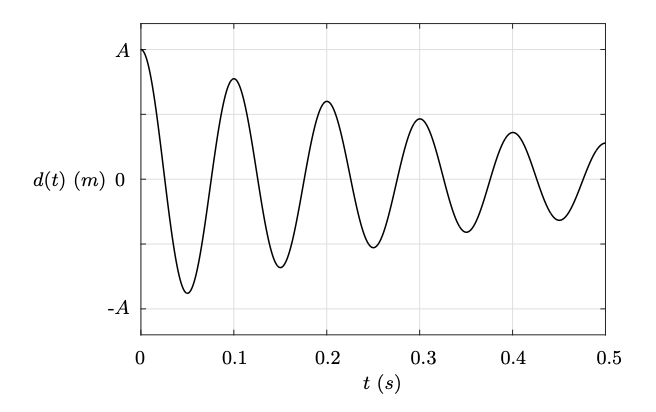
\includegraphics[width=0.5\linewidth]{./figures/f3_2_2.png}
\end{figure}

\paragraph{a)}
Determine the damping ratio $\xi$ and determine if the system is undercritically damped, critically damped or overcritically damped.
\bigbreak
The dampening ratio $\delta$ is defined as
\[ 
\delta \equiv \frac{1}{j} \log \left( \frac{d(t)}{d(t + jT_d)} \right)
.\]
Where $j \in \mathbb{N}_{>0}$ is chosen such that $t + jT_d$ is the time $j$ damped eigenperipds after $t$, where each eigenperiod is $T_d$. In this case we have:
\begin{align*}
  \delta &= \frac{1}{2} \ln \left( \frac{d(t)}{ \frac{3}{5} d(t)} \right) \\
  &= \frac{1}{2} \ln \frac{5}{3} \\
  &= \num{0,268} 
.\end{align*}
Hence:
\[ 
\xi = \frac{\delta}{\sqrt{\delta^2 + 4 \pi^2}} = \frac{\num{0,268} }{\sqrt{\num{0,268}^2 + 4 \pi^2}} = \num{0,042} 
.\]
Hence the system is undercritically damped. 



\paragraph{b)}
Determine the damped angular eigenfrequency $\omega_d$. (hint: look at the movement graph).
\bigbreak
From the plot we see that $T_d = \qty{0,1}{s}$, hence:
\[ 
\omega_d = \frac{2\pi}{T_d} = 20 \pi \unit{s^{-1}}
.\]


\paragraph{c)}
Determine the undamped angular eigenfrequency $\omega_u$.
\bigbreak
Here we have:
\[ 
\omega_u = \frac{\omega_d}{\sqrt{1 - \xi^2}} = \frac{20 \pi \unit{s^{-1}}}{\sqrt{1 - \num{0,042}^2}} \approx \qty{62,88}{s^{-1}}
.\]

\paragraph{d)}
It is noted that $m = \qty{2,2}{kg} $ and $k_1 = \qty{3000}{\frac{N}{m}} $. Determine $k_2$.
\bigbreak
We know that:
\[ 
k_{\mathrm{eq}} = k_1 + k_2
\]
as the springs are connected in parallel. We have that:
\[ 
\omega_u^2 = \frac{k_{\mathrm{eq}}}{m} = \frac{k_1 + k_2}{m} \implies k_2 = \omega_u^2 m - k_1
.\]
Plugging in known values we get:
\[ 
k_2 = \left( \qty{62,88}{s^{-1}}  \right)^2 \cdot \qty{2,2}{kg} - \qty{3000}{\frac{N}{m}} = \qty{5,7}{\frac{kN}{m}} 
.\]

